\chapter{Category Theory and Graph Grammars Basic Notions}\label{ch:gts}

\section{Category Theory}

\begin{definition}[Category] A category \cat{C} consists of a collection of \emph{objects} and a collection of \emph{arrows} between objects (also called \emph{morphisms}) such that:

  \begin{enumerate}
    \item for all arrows $f : A \rightarrow B$, $g : B \rightarrow C$ and
$h : C \rightarrow D$, with objects $A,B,C,D$ not necessarily distinct, the composition of arrows is associative:

  $h \circ (g \circ f) = (h \circ g) \circ f$;
    \item for every object $A$ there is an \emph{identity} arrow $id_A : A \rightarrow A$ such that for any arrow $f : A \rightarrow B$:

  $id_B \circ f = f$ and $f \circ id_A = f$.
  \end{enumerate}

\end{definition}

\begin{example}[Category Examples]
\end{example}

\begin{definition}[Diagram] Given a category \cat{C}, a diagram in \cat{C} is a collection of vertices and directed edges such that, if an edge in the diagram is named with an arrow $f$ and $f$ has domain $A$ and codomain $B$, then the outgoing vertice of the edge must be named $A$ and the incoming vertice $B$.

  A diagram is said to \emph{commute} if, for every pair of objects $A,B$, all the paths in the diagram from $A$ to $B$ are equal. In other words, each path in the diagram determines an arrow and these arrows are equal in \cat{C}. To say that the diagram bellow commutes is equal to say that \mbox{$g' \circ f = f' \circ g$}.

\diagram{
  A\ar[r]^{f}\ar[d]_{g} & Y\ar[d]^{g'}\\
  X\ar[r]_{f'} & B
}

\end{definition}

\begin{definition}[Monomorphism, Epimorphism and Isomorphism] An arrow \mbox{$f : B \rightarrow C$} in a category \cat{C} is said to be a \emph{monomorphism} if, for any pair of arrows $g : A \rightarrow B$ and $h : A \rightarrow B$, we have that $f \circ g = f \circ h \Rightarrow g = h$.

\diagram{
  A\ar@<.5ex>[r]^{g}\ar@<-.5ex>[r]_{h} & B\ar[r]^{f} & C
}

  An arrow \morph{f}{A}{B} is said to be an \emph{epimorphism} if, for any pair of arrows \morph{g}{B}{C}, \morph{h}{B}{C}, we have that \mbox{$g \circ f = h \circ f \Rightarrow g = h$}.

\diagram{
  A\ar[r]^{f} & B\ar@<.5ex>[r]^{g}\ar@<-.5ex>[r]_{h} & C
}

  An arrow \morph{f}{A}{B} is an \emph{isomorphism} if there is an arrow \morph{f^{-1}}{B}{A}, the \emph{inverse} of $f$, such that \mbox{$f^{-1} \circ f = id_A$} and \mbox{$f \circ f^{-1} = id_B$}


\diagram{ 
  A\ar@<.5ex>[r]^{f} & B\ar@<.5ex>[l]^{f^{-1}}
}
\end{definition}

\begin{example}[Monorphism, Epimorphism and Isomorphism Examples]
\end{example}


\subsection{Categorial Constructions}

Here we present basic categorial constructions that are used in this work. Notice that this is not an extensive list, we present only the ones necessary to our scope. For a more in-depth explanation of Categories and their applications in Computer Science see~\cite{Pierce1991}.\tinytodo{Give an intuitive notion of the constructions before defining it?}


\begin{definition}[Coproduct] Given two objects $A$ and $B$, their \emph{coproduct} (also called \emph{categorical sum}) is an object $A+B$ and two injection arrows \tinytodo{define injections?} \morph{i_1}{A}{A+B} and \morph{i_2}{B}{A+B} such that, for any other object $C$ an pair of arrows \morph{f}{A}{C} and \morph{g}{B}{C} there is one unique arrow \morph{!}{A+B}{C} such that the following diagram commutes:

\diagram{
  A\ar[r]^{i_1}\ar[dr]_{f} & A+B\ar@{.>}[d]^{!} & B\ar[l]_{i_2}\ar[dl]^{g}\\
    & C   &
}

  \begin{example}[Coproducts in \cat{Set}] In the category \cat{Set}, the coproduct construction generalizes the notion of disjoint union. \tinytodo{draw example}

    It also generalizes the notion of disjoint union in the category \cat{Graph}. \tinytodo{draw examples}
\end{example}

\end{definition}

\begin{definition}[Coequalizer] Given two objects $A$ and $B$ with two parallel morphisms \morph{f}{A}{B} \morph{g}{A}{B}, the coequalizer of the diagram is an object $X$ together with a morphism \morph{h}{B}{X} such that \mbox{$h \circ f = h \circ g$} and, for any other such objects $X'$ with a morphism $h'$, there is a unique morphism \morph{!}{X}{X'} such that the following diagram commutes.

\diagram{
  A\ar@<.5ex>[r]^{f}\ar@<-.5ex>[r]_{g} & B\ar[r]^{h}\ar[dr]_{h'} & X\ar@{.>}[d]^{!}\\
    &   & X'
}
\end{definition}

\begin{example}[Coequalizers in \cat{Set}] In the categories \cat{Set} and \cat{Graph} ,the coequalizer generalizes the notion of smallest equivalence relation. \tinytodo{draw examples}.
\end{example}

\begin{definition}[Colimit] Given a diagram $D$ in a category \cat{C}, a \emph{cocone} for $D$ is an object $X$ and a family of morphisms \morph{f_i}{D_i}{X} (one for each object $D_i$ in $D$), such that for each morphism $g$ in $D$ the outer part of the following diagram commutes.

\diagram{
  D_i\ar[rr]^{g}\ar[dr]_{f_i} &   & D_j\ar[dl]^{f_j}\\
      & X &   \\
}
\hfill

  A \emph{colimit} for a diagram $D$ is a cocone \{\morph{f_i}{D_i}{X}\} such that for any other cocone \{\morph{f'_i}{D'_i}{X'}\} there exists a unique morphism \morph{!}{X}{X'} such that the following diagram commutes for every $D_i$ in $D$.


\diagram{
  D_i\ar@/_1.1pc/[ddr]_{f'_i}\ar[rr]^{g}\ar[dr]_{f_i} &   & D_j\ar@/^1.1pc/[ddl]^{f'_j}\ar[dl]^{f_j}\\
      & X\ar@{.>}[d]^{!} &   \\
      & X'&    \\
}
\end{definition}

\begin{example}[Colimits in \cat{Set}]
\end{example}

\begin{definition}[Pushout] Pushouts are a special case of colimits. Given a span of arrows \mbox{$B \xleftarrow{f} A \xrightarrow{g} C$}, its \emph{pushout} is an object $X$ together with a pair of arrows \morph{f'}{C}{X} and \morph{g'}{B}{X} such that (1) \mbox{$f' \circ g = g' \circ f$} and (2) for any other object $X'$ with morphisms \morph{i}{B}{X'} and \morph{j}{C}{X'} such that $i \circ f = j \circ g$ there is a unique morphism \morph{!}{X}{X'} such that \mbox{$i =$ $! \circ g'$} and \mbox{$j =$ $! \circ f'$}.

\diagram{
  A\ar[r]^{f}\ar[d]_{g} & B\ar[d]^{g'}\ar@/^1.1pc/[rdd]^{i} &\\
  C\ar[r]_{f'}\ar@/_1.1pc/[drr]_{j}       & X\ar@{.>}[dr]^{!}&\\
                &         &X'
}

\end{definition}

\begin{example}[Pushouts in \cat{Set}]
\end{example}

\iffalse
\begin{definition}[Pullback] \tinytodo{Maintain only if we are going to use the concurrent rules chapter} Given 

\diagram{
  X'\ar@{.>}[dr]^{!}\ar@/^1.1pc/[rrd]^{i}\ar@/_1.1pc/[ddr]_{j}  & &\\
  & X\ar[r]^{g'}\ar[d]_{f'} & B\ar[d]^{f}\\
  & C\ar[r]_{g}      & A
}
\end{definition}

\begin{example}[Pullbacks in \cat{Set}]
\end{example}
\fi

\section{Graph Grammars}

The theory of graph grammars and graph transformation systems is based on the application of rules that are able to modify graphs. Using this framework, it is possible to model complex systems as graph transformation systems, where graphs represent the system states and the rules model transitions between states.

Graph grammars have a wide application in computer science, not only because graphs are very natural and intuitive way to model complex situations, but also because it is possible to reason about several properties of the modelled systems using the its formalism~\cite{Ehrig2006, Ehrig1999handbook}.

\begin{definition}[Graph] A graph is a tuple $G = \left(V,E,s,t\right)$ where: $V$ is a set of nodes, $E$ is a set of Edges and $s,t : E \rightarrow V$ are two total functions that map each edge in $E$ to its source and target in $V$.

\end{definition}

\begin{example}[Graph] Figure~\ref{fig:gts:graph} shows a simple graph $G$ with $V = \{1,2,3,4\}$, $E = \{1,2\}$, $s =\{(1,1),(2,3)\}$ and $t = \{(1,2),(2,3)\}$.
\begin{figure}[!ht]
  \centering
  
\includegraphics[scale=0.8]{images/gts/graph}
  \caption{A graph example}\label{fig:gts:graph}
\end{figure}
\end{example}

\begin{definition}[Graph Morphism] Given two graphs $G_1,G_2$ with $G_i = \left(V_i, E_i, s_i, t_i\right)$ for $i$ in $[1,2]$, a graph morphism $f : G_1 \rightarrow G_2$ between them is a pair $f = \left(f_V,f_E\right)$ where $f_V : V_1 \rightarrow V_2$ and $f_E : E_1 \rightarrow E_2$ are total functions that preserve the source and target functions, i.e. $f_V \circ s_1 = s_2 \circ f_E$ and $f_V \circ t_1 = t_2 \circ f_E$. \tinytodo{Talk about injective / surjective / isomorphic morphisms?} \tinytodo{Talk about morphisms composition?}
\end{definition}

\begin{example}[Graph Morphisms]Figure~\ref{fig:gts:compact-graph-morphism} shows three morphisms $f : G_0 \rightarrow G_1$, $g : G_0 \rightarrow G_2$ and $h : G_0 \rightarrow G_3$, which are a monomorphism, an epimorphism and a isomorphism, respectively.

  The morphism $f$ maps node $\Circle_1$ to $\Circle_a$, node $\Circle_2$ to $\Circle_b$ and edge $\curvearrowleft_1$ to $\curvearrowleft_q$; $g$ maps both nodes $\Circle_1$ and $\Circle_2$ to $\Circle_c$ and edge $\curvearrowleft_1$ to $\curvearrowleft_r$; and $h$ maps node $\Circle_1$ to $\Circle_d$, node $\Circle_2$ to $\Circle_e$ and edge $\curvearrowleft_1$ to $\curvearrowleft_s$.

  Figure~\ref{fig:gts:expanded-graph-morphism} shows the morphism $f$ in an expanded (explicit) notation. Both notations will be used through this work according to which one will be the better to clarify the meaning at the moment.
\begin{figure}[!ht]
  \centering
  \fbox{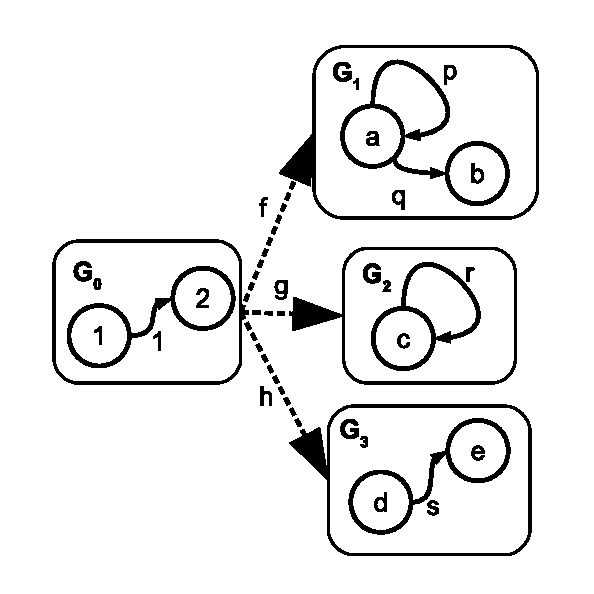
\includegraphics[scale=0.8]{images/gts/compact-graph-morphism}}
  \caption{A graph morphism example}\label{fig:gts:compact-graph-morphism}
\end{figure}

\begin{figure}[!ht]
  \centering
  \fbox{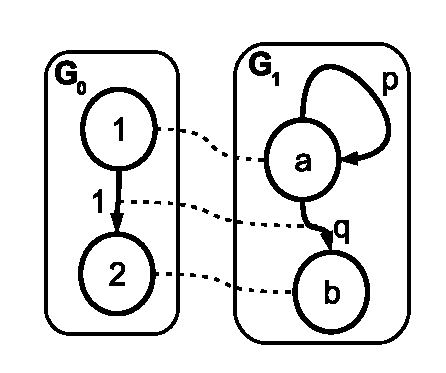
\includegraphics[scale=0.8]{images/gts/expanded-graph-morphism}}
  \caption{An expanded graph morphism example}\label{fig:gts:expanded-graph-morphism}
\end{figure}
\end{example}

\begin{definition}[Typed Graph and Typed Graph Morphism] A type graph is a distinguished graph $TG = \left(V_{TG},E_{TG},s_{TG},t_{TG}\right)$ where $V_{TG}$ and $E_{TG}$ are called the node and edge type alphabets, respectively.

  A typed graph is a pair $G^T = \left(G, type\right)$ consisting of a graph $G$ and a graph morphism $type : G \rightarrow TG$.

  Given two typed graphs $G^T_1 = \left(G_1,type_1\right)$ and $G^T_2 =\left(G_2,type_2\right)$, a typed graph morphism $f : G^T_1 \rightarrow G^T_2$ is a graph morphism $f : G_1 \rightarrow G_2$ such that $type_2 \circ f = type_1$:

\diagram{
  G_1\ar[rr]^{f}\ar[dr]_{type_1} & & G_2\ar[dl]^{type_2}\\
  \ar@{}[rur]|{=}& TG &
}
  \tinytodo{Talk about he category of graphs typed over T}
\end{definition}

\begin{example}[Typed Graph and Typed Graph Morphism Example] Figure~\ref{fig:gts:typed-graphs} shows a type graph $T$, and four graphs $G_0, G_1, G_2, G_3$ where only $G_0$ and $G_1$ are valid \emph{T-typed} graphs. 
  
  Notice that $G_2$ can not be a \emph{T-typed} graph because type graph does not have a node of the type $\lozenge$, neither an edge type with source and target in the $\Square$ type. Similarly, $G_3$ is not a valid \emph{T-typed} graph because, although there is an edge type between a $\triangle$ and a $\Square$ types, the source must of this type of edge must be a $\Square$ and the target a $\triangle$.

  Figure~\ref{fig:gts:typed-graph-morphism} shows a typed graph morphism $f : G_0^T \rightarrow G_1^T$, where $f$ maps node $\Circle_a$ to $\Circle_1$, $\Square_b$ to $\Square_1$ and edge $\curvearrowleft_e$ to $\curvearrowleft_2$.
\begin{figure}[!ht]
  \centering
  \fbox{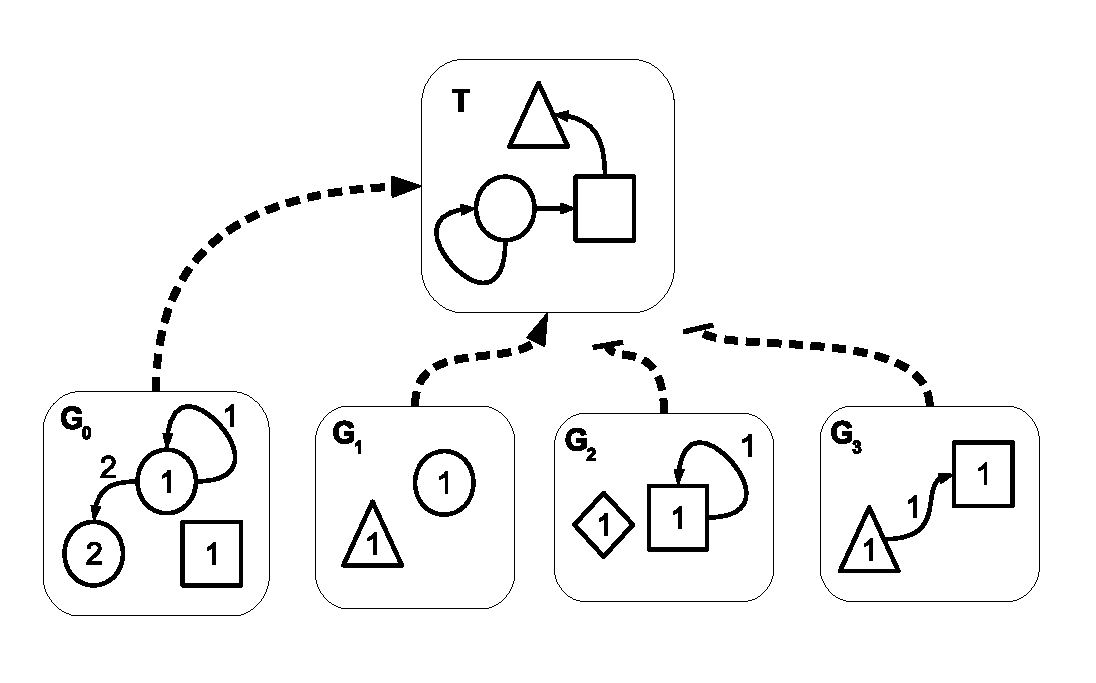
\includegraphics[scale=0.65]{images/gts/typed-graphs}}
  \caption{\emph{T-typed} valid and invalid graphs}\label{fig:gts:typed-graphs}
\end{figure}

\begin{figure}[!ht]
  \centering
  \fbox{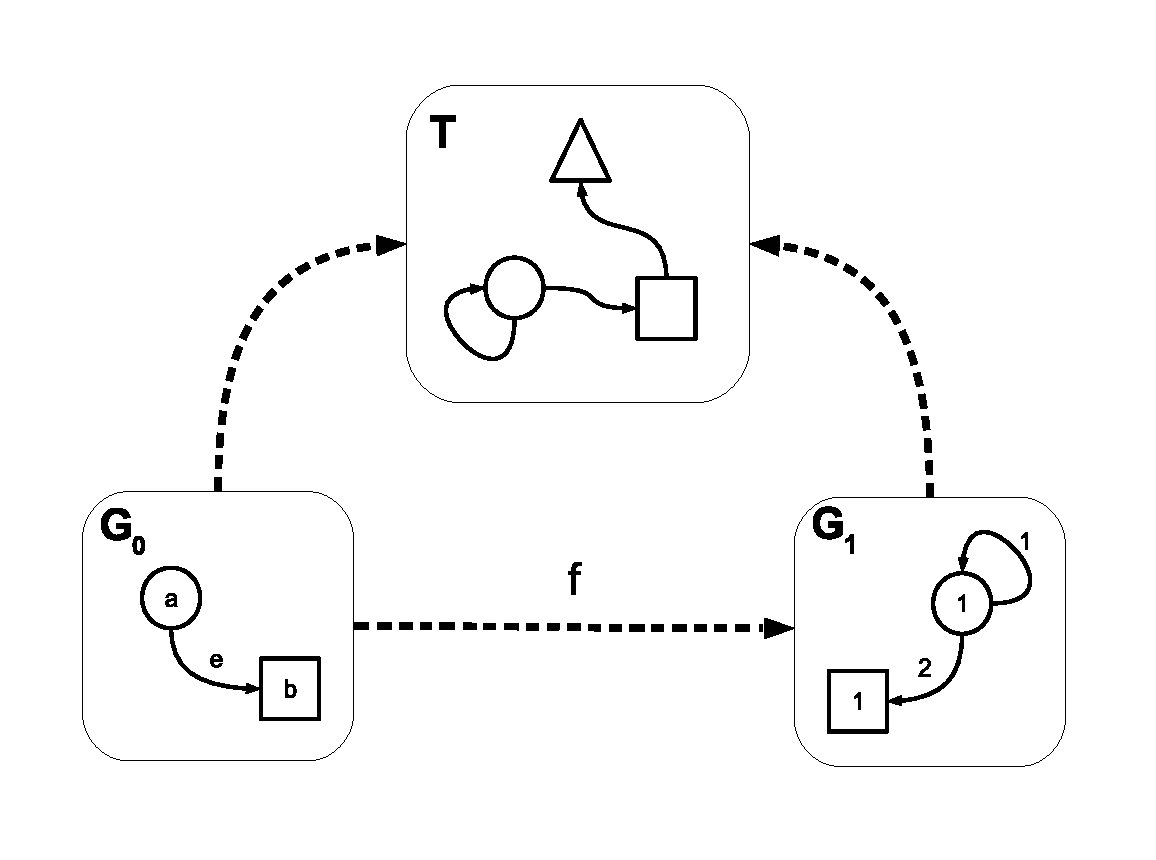
\includegraphics[scale=0.6]{images/gts/typed-graph-morphism}}
  \caption{A typed graph morphism}\label{fig:gts:typed-graph-morphism}
\end{figure}
\end{example}

\begin{definition}[Positive Atomic Constraint] A \emph{positive} atomic (typed) graph constraint is of the form $PC\left(a\right)$, where $a : P \rightarrow C$ is a (typed) graph morphism. A (typed) graph $G$ satisfies $PC\left(a\right)$ if for every injective (typed) graph morphism $p : P \rightarrow G$ there is at least one injective (typed) graph morphism $q : P \rightarrow C$ such that $p = q \circ a$.

  A positive (typed) graph constraint with $a : \emptyset \rightarrow C$ is also notated $PC\left(C\right)$. Given a (typed) graph $G$, it satisfies $PC\left(C\right)$ if there is an injective (typed) graph morphism $q : C \rightarrow  G$.
\diagram{
  P\ar[rr]^{a}\ar[dr]_{p} & & C\ar[dl]^{q}\\
  \ar@{}[rur]|{=}& G &
}

\end{definition}

\begin{definition}[Negative Atomic Constraint]
A \emph{negative} atomic (typed) graph constraint is of the form $NC\left(a\right)$, where $a : P \rightarrow C$ is a (typed) graph morphism. A (typed) graph $G$ satisfies $PC\left(a\right)$ if for every injective (typed) graph morphism $p : P \rightarrow G$ there is no injective (typed) graph morphism $q : P \rightarrow C$ such that $p = q \circ a$.

  A negative (typed) graph constraint with $a : \emptyset \rightarrow C$ is also notated $NC\left(C\right)$. Given a (typed) graph $G$, it satisfies $NC\left(C\right)$ if there is no injective (typed) graph morphism $q : C \rightarrow G$.

\diagram{
  P\ar[rr]^{a}\ar[dr]_{p} & & C\ar[dl]|{|}^{q}\\
  \ar@{}[rur]|{=}& G &
}

\end{definition}

\begin{remark} It was shown in ~\cite{Ehrig2006} that negative atomic constraints do not give more expressive power. However, we introduced this concept because it makes easier to reason about some of the purposes of this thesis in a negative rather than a positive manner.\tinytodo{related to the graph constraint definition, maybe this is not necessary}
\end{remark}

\begin{definition}[Graph Constraint] A (typed) graph constraint is a \emph{boolean} formula over atomic (typed) graph constraints, in such way that $true$, $false$ and every atomic constraint are also graph constraints. Also, if $c$ and $c_i$, with $i \in I$ for some index set $I$, are graph constraints, then $\neg c$, $\land_{i \in I} c_i$ and $\lor_{i \in I} c_i$ are also graph constraints.

  A graph $G$ satisfies a graph constraint $c$ (written $G \models c$) iff one of the following situations occurs:
  \begin{itemize}
    \item $c = true$
    \item $c$ is an atomic constraint $a$ and $G \models a$
    \item $c = \neg c'$ and $G \not\models c'$
    \item $c = \land_{i \in I}c_i$ and $G \models c_i$ $\forall i \in I$ 
    \item $c = \lor_{i \in I}c_i$  and $\exists i \in I$ such that $G \models c_i$
  \end{itemize}
\end{definition}

\begin{example}[Constraints Example]
\end{example}

\begin{definition}[Graph Rule]\label{def:graph-rule} A (typed) graph rule\footnote{Also called graph transformation rule or graph production.} \graphrule{} is a span of injective (typed) graph morphisms \lefthand{} and \righthand{}  where the (typed) graphs $L$, $K$ and $R$ are called the left-hand side, gluing graph and right-hand side, respectively.

  Given a (typed) graph rule $p$, its inverse rule is defined by \inversegraphrule.
\end{definition}

\begin{example}[Graph Rule Example and Notation] Figure~\ref{fig:gts:rule} shows an example of a graph rule which reads a node of the type $\Circle$, deletes a node of the type $\triangle$ and then creates a node of the type $\Square$ with an edge between the $\Circle$ and the \Square. 
  
Figure ~\ref{fig:gts:rule-standard} presents the rule in the standard DPO notation, while Figure~\ref{fig:gts:rule-compact} depicts the same rule in a compact notation, where the gluing graph is omitted. 

Sometimes we will use the compact notation to make the figures smaller. Notice that the compact notation does not cause any loss as the gluing graph can be obtained as the ``intersection'' of the left and right graphs, and the morphisms $l$ and $r$ as the inclusions of $K$ in $L$ and $R$, respectively.

\begin{figure}[!ht]
  \centering
  \begin{subfigure}[t]{.5\textwidth}
    \centerline{\fbox{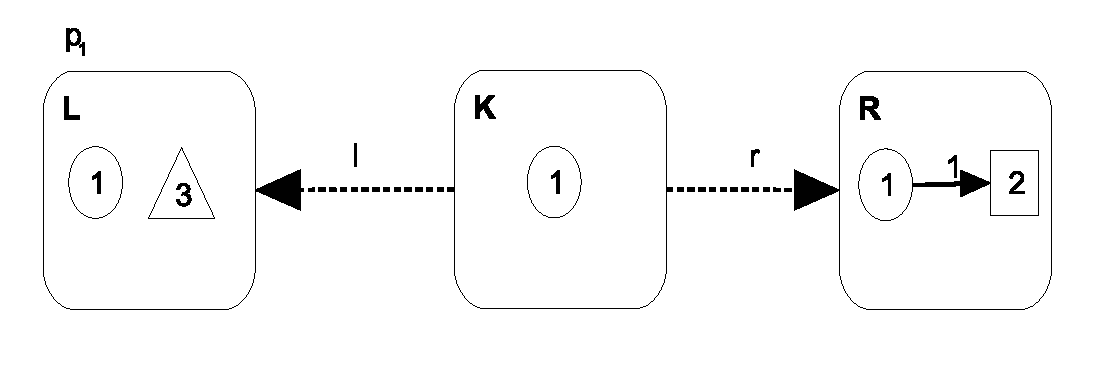
\includegraphics[scale=0.5]{images/gts/standard-dpo-rule}}}
    \caption{Standard DPO rule notation}\label{fig:gts:rule-standard}
  \end{subfigure}

  \begin{subfigure}[t]{.5\textwidth}
    \centerline{\fbox{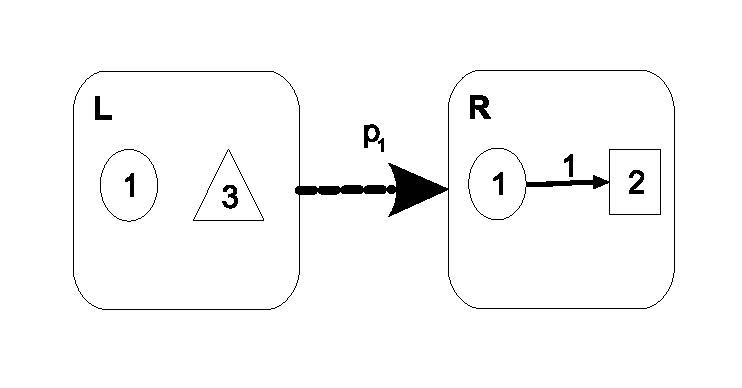
\includegraphics[scale=0.5]{images/gts/compact-dpo-rule}}}
    \caption{Compact DPO rule notation}\label{fig:gts:rule-compact}
  \end{subfigure}
  \caption{DPO graph rule}\label{fig:gts:rule}
\end{figure}
\end{example}

\begin{definition}[Graph Transformation] Given a (typed) graph rule \graphrule{} and a (typed) graph $G$ with a (typed) graph morphism \match, called match, a direct (typed) graph transformation $G \xRightarrow{p,m} H$ from $G$ to a (typed) graph $H$ is a double-pushout (DPO) diagram such as:\tinytodo{Explain gluing conditions.}

\diagram{
  L\ar[d]_{m}        & & K\ar[ll]_{l}\ar[rr]^{r}\ar[d]|{k} & & R\ar[d]^{m'}\\
  G\ar@{}[urr]|{\left(1\right)} & & D\ar[ll]^{f}\ar[rr]_{g}             & & H\ar@{}[ull]|{\left(2\right)}
}
\end{definition}

\begin{example}[Graph Transformation Examples] Figure~\ref{fig:gts:transformation-success} shows a transformation where the rule depicted in Figure~\ref{fig:gts:rule} is successfully applied over a graph instance $G_0$.

  Figure~\ref{fig:gts:transformation-fail} shows the same rule being applied over a graph instance $G_1$ which does not satisfy the gluing conditions (more specifically the dangling condition), therefore the transformation can not be applied as the result would not be a valid graph.

\begin{figure}[!ht]
  \centering
  \begin{subfigure}[t]{.5\textwidth}
    \centerline{\fbox{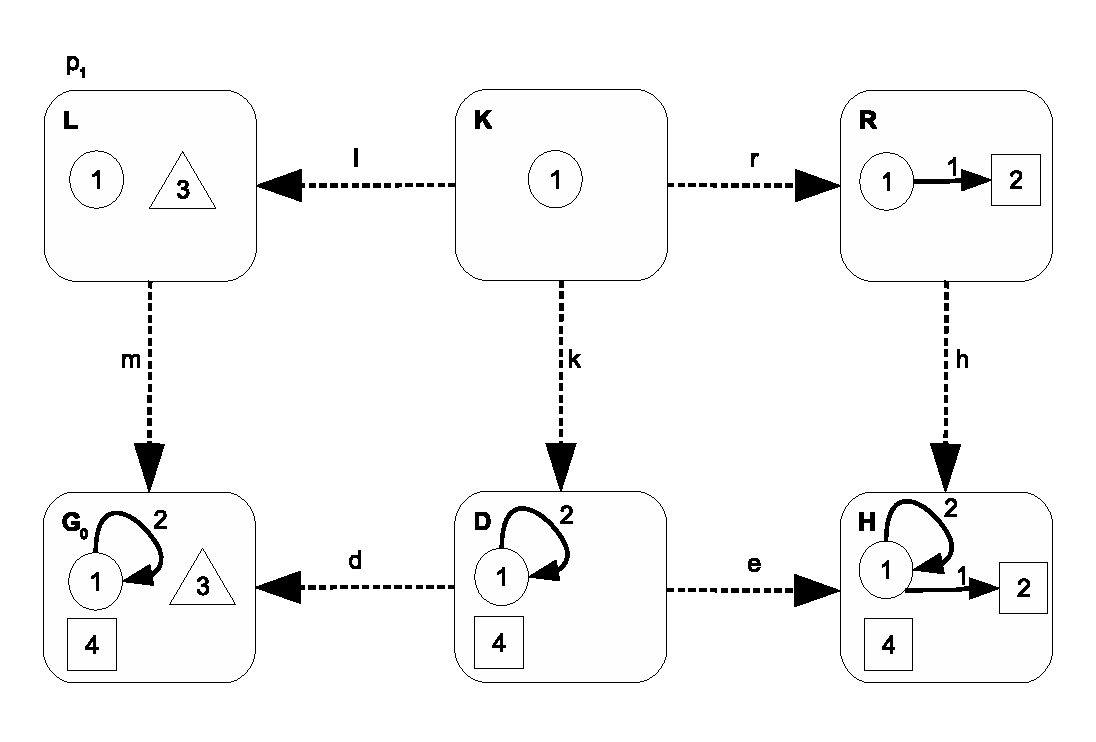
\includegraphics[scale=0.8]{images/gts/transformation}}}
    \caption{Successfully applied graph transformation}\label{fig:gts:transformation-success}
  \end{subfigure}

  \begin{subfigure}[t]{.5\textwidth}
    \centerline{\fbox{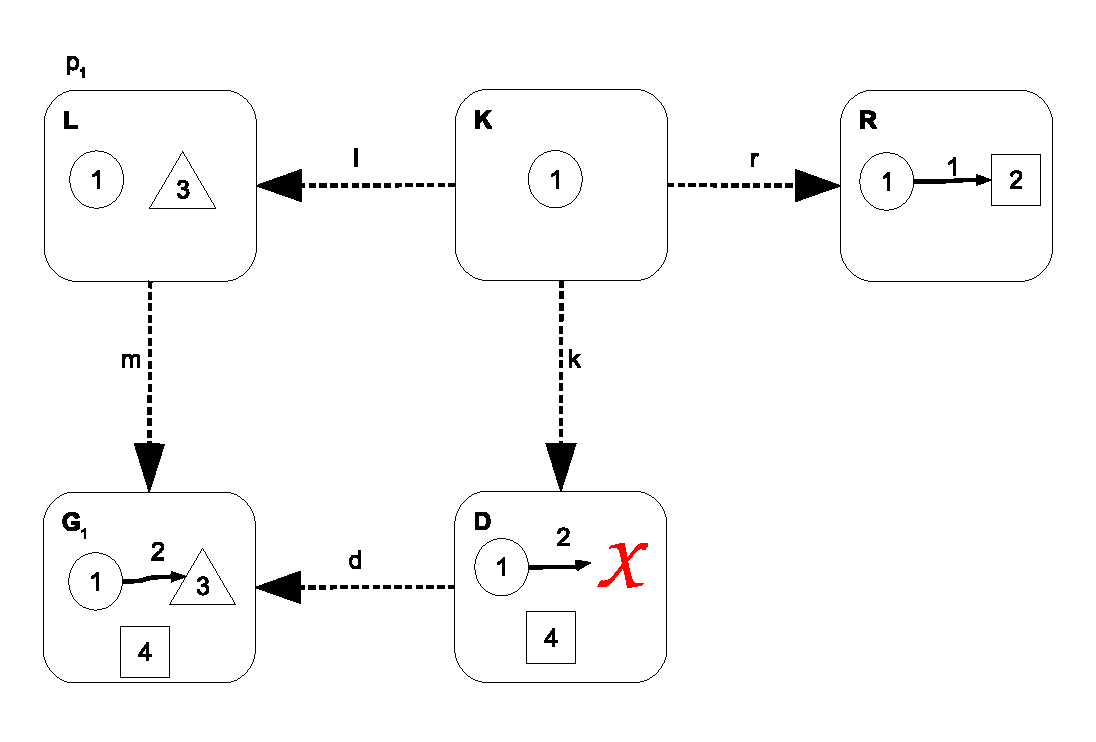
\includegraphics[scale=0.8]{images/gts/transformation-failed}}}
    \caption{Failing graph transformation due to the dangling condition}\label{fig:gts:transformation-fail}
  \end{subfigure}
  \caption{Graph transformation}\label{fig:gts:transformation}
\end{figure}

\end{example}
\begin{definition}[Negative Application Condition] A \emph{left} negative application condition over a graph rule \graphrule{} is of the form $NAC\left(n\right)$, where \nac{} is an arbitrary (typed) graph morphism. A match \match{} of a rule $p$ satisfies\footnote{When a NAC is satisfied it is also said that the NAC is \emph{not triggered} and vice versa.} $NAC\left(n\right)$ on $L$, written $m \models NAC\left(n\right)$, iff $\nexists$ $q : N \rightarrow G$ with $q$ injective and $q \circ n = m$.

\diagram{
  N\ar@{.>}[dr]|{|}_{q} & L\ar[d]^{m}\ar[l]_{n}\\
   & G
}

  A match \match{} satisfies a set \mbox{$NAC_L = \{NAC\left(n_i\right)|i \in I\}$} of left $NACs$, iff \mbox{$m \models NAC\left(n_i\right)$} $\forall i \in I$.

  Analogously, a \emph{right} negative application condition over a graph rule \graphrule{} is of the form $NAC\left(n\right)$, where \rightnac{} is an arbitrary (typed) graph morphism. A comatch \comatch{} of a rule $p$ satisfies $NAC\left(n\right)$ on $R$ (written \mbox{$m' \models NAC\left(n\right)$}) iff $\nexists$ $q : N \rightarrow H$ with $q$ injective and $q \circ n = m'$.

\diagram{
  R\ar[d]_{m'}\ar[r]^{n} & N\ar@{.>}[dl]|{|}^{q}\\
  H &
}
  Also, a comatch \comatch{} satisfies a set \mbox{$NAC_R = \{NAC\left(n_i\right)|i \in I\}$} of right $NACs$, iff $m' \models NAC\left(n_i\right)$ $\forall i \in I$.

\end{definition}

\begin{example}[NAC and NAC satisfiability] Figure~\ref{fig:gts:nacs:satisfied} shows a NAC that is satisfied (i.e. not triggered) over a match $m$, as there is no possible way of mapping the edge between $\Circle_1$ and $\Square_1$ in $N$ to an edge in $G_0$ such that the resulting triangle commutes. Therefore, if $G_0$ also satisfies the gluing conditions for the corresponding rule the transformation can be applied.

  On the other hand, Figure~\ref{fig:gts:nacs:triggered} shows a NAC that is triggered (i.e. not satisfied) over the match $m$: all the elements in $N$ can be mapped to $G_0$ such that the resulting triangle commutes. Therefore, even if $G_0$ satisfies the gluing conditions, the transformation can never be applied, as the forbidden pattern of the NAC was found on the instance graph.
  
\begin{figure}[!ht]
  \centering
  \begin{subfigure}[t]{.5\textwidth}
    \centerline{\fbox{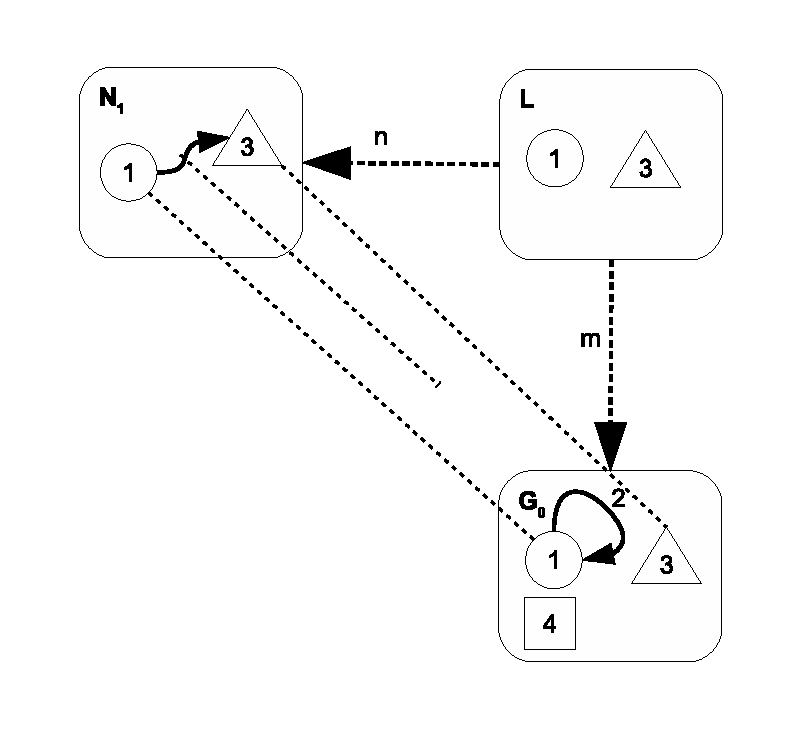
\includegraphics[scale=0.55]{images/gts/satisfied_nac}}}
    \caption{A satisfied NAC}\label{fig:gts:nacs:satisfied}
  \end{subfigure}%
  \begin{subfigure}[t]{.5\textwidth}
    \centerline{\fbox{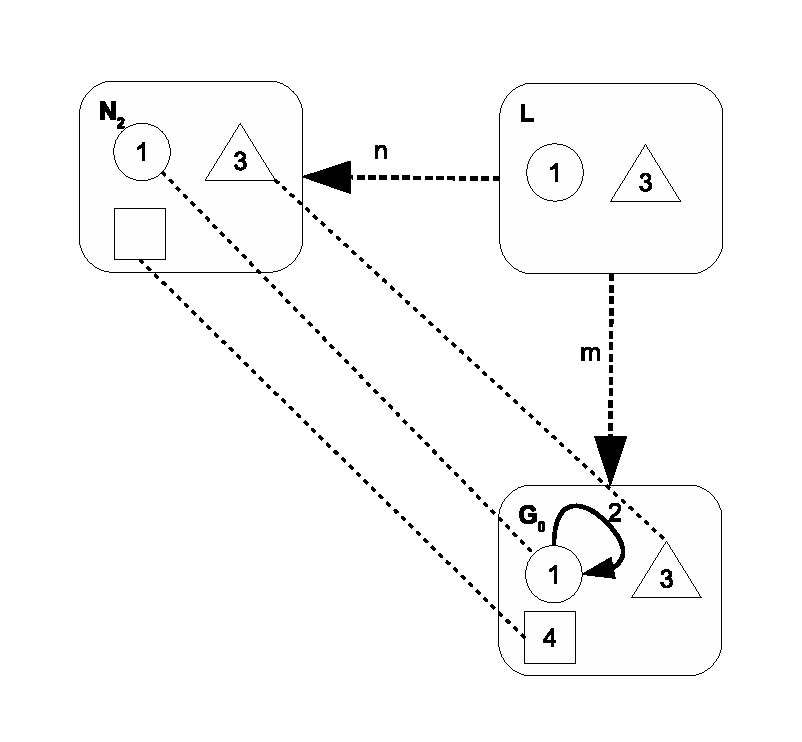
\includegraphics[scale=0.55]{images/gts/triggered_nac}}}
    \caption{A triggered NAC}\label{fig:gts:nacs:triggered}
  \end{subfigure}
  \begin{subfigure}[t]{.5\textwidth}
    \centerline{\fbox{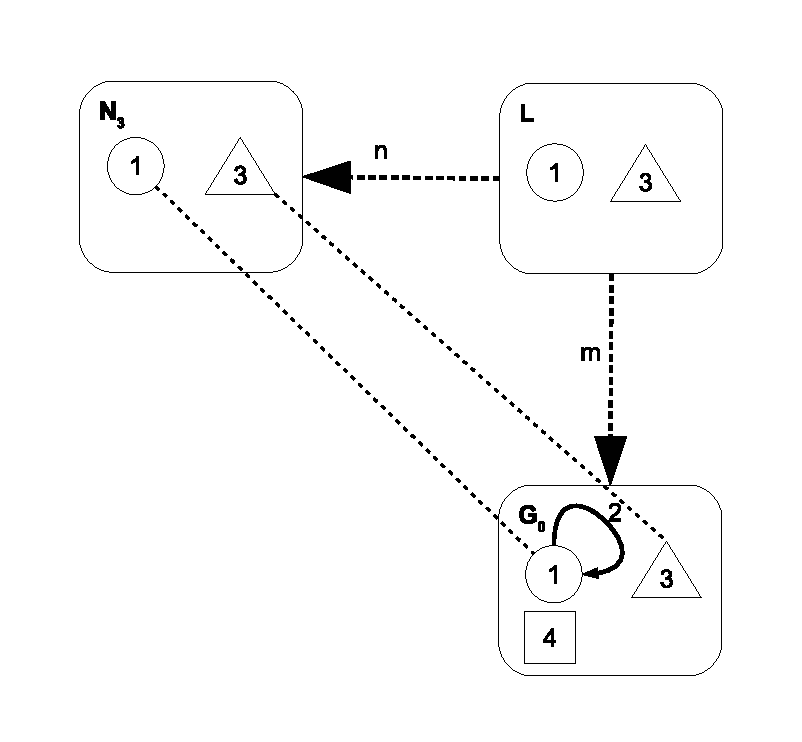
\includegraphics[scale=0.55]{images/gts/trivially_triggered_nac}}}
    \caption{A trivially-triggered NAC}\label{fig:gts:nacs:trivial}
  \end{subfigure}
  \caption{NACs and NAC satisfiability}\label{fig:gts:nacs}
\end{figure}
\end{example}

\begin{assumption}[Left NACs] Unless stated otherwise, we will work with graph rules that have only left $NACs$ for the rest of this thesis. This is without loss of generality once right $NACs$ can be translated to left ones as it is shown in Definition~\ref{def:shift-nac}.
\end{assumption}

\begin{definition}[Trivially-Triggered NACs] \tinytodo{explain that this occurs only with injective matches} Given a $NAC(n)$, where $n : L \rightarrow \hat{L}$ is a isomorphism, we call $NAC(n)$ a \emph{trivially-triggered NAC} as for each match \match{} there will always exist a $q : \hat{L} \rightarrow G$ injective such that $q \circ n = m$.

  A trivially-triggered NAC $n : L \rightarrow \hat{L}$ is also notated $NAC(L)$. If a rule $p$ has a trivially-triggered NAC then $p$ can never be applied whatsoever, as the NAC will never be satisfied. An example of a trivially-triggered NAC is shown on Figure~\ref{fig:gts:nacs:trivial}.
\end{definition}

\begin{definition}[Graph Transformation System and Graph Grammar] A typed graph transformation system is a pair $GTS = \left(TG,P\right)$ where $TG$ is the type graph of the system and $P$ is a set of typed graph rules with NACs.

  A typed graph grammar is a pair $GG = \left(GTS,S\right)$ where $GTS$ is a typed graph transformation system and $S$ is a typed start graph.
\end{definition}

\section{Parallel and Sequential Independence}

One of the characteristics that make Graph Transformation Systems and Graph Grammars suitable formalisms to model and reason about parallel and/or concurrent systems is the possibility to check whether two graph rules (or two graph transformations) can be applied together at the same time (parallel independence) or in any interchangeable order (sequential independence).

In this section, we show both what it means for two graph rules (graph transformations) to be independent and how to check it. Notice that when we are reasoning about graph transformations the (in)dependence is concrete, while for the case of graph rules the (in)dependence is potential, as it would depend on a particular pattern being found on an instance graph.

\begin{definition}[Causal Dependency]\label{def:classic-dependency} Given two graph rules $p_1,p_2$ with NACs, they are \emph{causally dependent} for a given graph $E$ in which they overlap iff one of the following situations occur in the diagram where all the squares are pushouts of the DPO rewriting: \tinytodo{change explanation to use graph transformations instead of graph rules?}

  \begin{enumerate}
    \item $\nexists h_{12} : R_1 -> D_2$ such that $d_2 \circ h_{12} = m_1'$
    \item $\exists! h_{12} : R_1 -> D_2$ such that $d_2 \circ h_{12} = m_1'$ but $e_2 \circ h_{12} \not\models NAC_{p_1^{-1}}$
    \item $\nexists h_{21} : L_2 -> D_1$ such that $e_1 \circ h_{21} = m_2$
    \item $\exists! h_{21} : L_2 -> D_1$ such that $e_1 \circ h_{21} = m_2$ but $d_1 \circ h_{21} \not\models NAC_{p_2}$
  \end{enumerate}

\diagram{
    N_1 & & & & N_2 & & \\
      L_1\ar[d]\ar[u]^{n_1} & K_1\ar[d]\ar[l]\ar[r] & R_1\ar[dr]_{m'_{1}}\ar@{.>}@/^1.1pc/[drrr]|<<{|}^<<<{h_{12}} & & L_2\ar[dl]^{m_2}\ar[u]^{n_2}\ar@{.>}@/_1.1pc/[dlll]|<<{|}_<<<{h_{21}} & K_2\ar[d]\ar[l]\ar[r] & R_2\ar[d]\\
        H_1 & D_1\ar[l]^{d_1}\ar[rr]_{e_1} & & \textit{E} & & D_2\ar[ll]^{d_2}\ar[r]_{e_2} & H_2\\
          & & & & & &
          }
\end{definition}

Intuitively, each dependency case can be regarded as follows:

\begin{enumerate}
  \item a \emph{deliver-delete} dependency: $p_2$ deletes (from graph $E$) at least one element that was created or preserved by $p_1$.
  \item a \emph{forbid-produce} dependency: $p_2$ creates on $H_2$ at least one element that would trigger the NAC $N_1^{-1}$.
  \item a \emph{produce-use} dependency: $p_1$ creates (on graph $E$) at least one element needed for $p_2$ to be applied which did not exist on $H_1$.
  \item a \emph{delete-forbid} dependency: $p_1$ deletes (from graph $H_1$) at least one element that would trigger the NAC $N_2$, thus allowing the application of $p_2$ on $E$.
\end{enumerate}

\begin{definition}[Conflict]\label{def:classic-conflict} Given two graph rules $p_1, p_2$ with NACs they are in conflict for a given graph $E$ in which they overlap iff one of the following situations occur:

\begin{enumerate}
    \item $\nexists h_{12} : L_1 -> D_2$ such that $d_2 \circ h_{12} = m_1$
    \item $\exists! h_{12} : R_1 -> D_2$ such that $d_2 \circ h_{12} = m_1$ but $e_2 \circ h_{12} \not\models NAC_{p_1}$
    \item $\nexists h_{21} : L_2 -> D_1$ such that $d_1 \circ h_{21} = m_2$
    \item $\exists! h_{21} : L_2 -> D_1$ such that $d_1 \circ h_{21} = m_2$ but $e_1 \circ h_{21} \not\models NAC_{p_2}$
  \end{enumerate}

\diagram{
     & & N_1 & & N_2 & & \\
      R_1\ar[d] & K_1\ar[d]\ar[l]\ar[r] & L_1\ar[u]^{n_1}\ar[dr]^{m_1}\ar@{.>}@/^1.1pc/[drrr]|<<{|}^<<<{h_{12}} & & L_2\ar[dl]_{m_2}\ar[u]^{n_2}\ar@{.>}@/_1.1pc/[dlll]|<<{|}_<<<{h_{21}} & K_2\ar[d]\ar[l]\ar[r] & R_2\ar[d]\\
        H_1 & D_1\ar[l]^{e_1}\ar[rr]_{d_1} & & \textit{E} & & D_2\ar[ll]^{d_2}\ar[r]_{e_2} & H_2\\
          & & & & & &
          }
\end{definition}

Intuitively, each conflict case can be regarded as:

\begin{enumerate}
  \item a \emph{delete-use} conflict: $p_2$ deletes (from graph $E$) at least one element needed for $p_1$ to be applied.
  \item a \emph{produce-forbid} conflict: $p_2$ produces (on graph $H_2$) at least one element that triggers the NAC $N_1$.
  \item a \emph{delete-use} conflict: $p_1$ deletes at least one element needed for $p_2$ to be applied
  \item a \emph{produce-forbid} conflict: $p_1$ creates at least one element that triggers the NAC $N_2$.
\end{enumerate}
